\documentclass{beamer}
\usepackage{graphicx}
\usepackage{grffile}
\usetheme[progressbar=frametitle]{metropolis}
\setbeamertemplate{frame numbering}[fraction]
%\useoutertheme{metropolis}
%\useinnertheme{metropolis}
\usefonttheme{metropolis}
\usecolortheme{spruce}
\setbeamercolor{background canvas}{bg=white}

\definecolor{mygreen}{rgb}{.125, .5,.25}
\usecolortheme[named=mygreen]{structure}

\title[Short Title]{Network Programming}
\subtitle{Design and Analysis}
\author{Dinh Anh Dung - 20140774 \\ An Nguyen Quynh Anh - 20140028 \\ Do Nhat Quang - 20140864}
\institute{\large \textbf{Hanoi University of Science and Technology}}
\date{}

\begin{document}

\begin{frame}
\titlepage
\end{frame}

\begin{frame}{Content}
	\tableofcontents
\end{frame}
\section{Application Introduction}
\begin{frame}{Application Introduction}
Our Application is about chatting program:

\begin{itemize}
\item Application require login and logout
\item Allow users to chat with each other
\item Allow users to create a group
\item Allow user to chat in a group
\item Allow user to send pictures to others
\end{itemize}
\end{frame}


\begin{frame}
\begin{columns}
\column{0.5\textwidth}
\begin{itemize}
\item Transport protocol TCP
\item Server - Client Architecture
\end{itemize}
\column{0.5\textwidth}
\begin{figure}
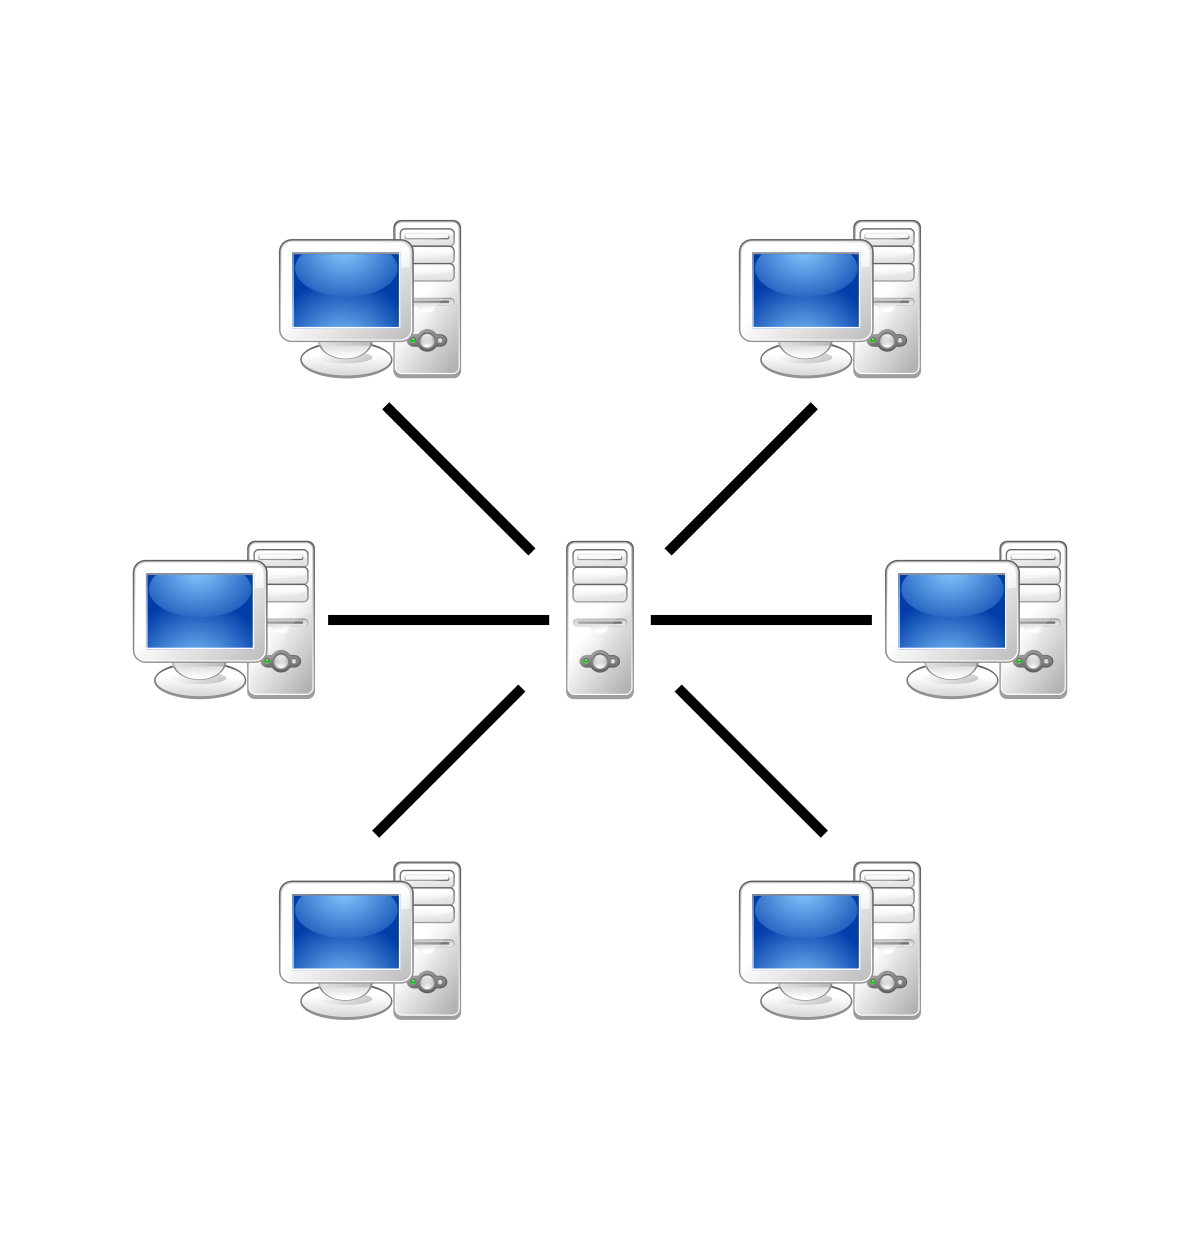
\includegraphics[scale=0.15]{1200px-Server-based-network.svg.png}
\caption{Model}
\end{figure}
\end{columns}
\end{frame}


\section{Design}
\begin{frame}{Design}
\begin{enumerate}
\item \textbf{Message Format}
\item \textbf{Modules}
\item \textbf{Protocol}
\end{enumerate}
\end{frame}


\subsection{Protocol Design}
\begin{frame}{Message Format}
\begin{enumerate}
\item Using JSON Format
\item Client message
\item Server Message
\end{enumerate}
\end{frame}


\begin{frame}{Client Message}
\begin{enumerate}
\item Method 
\item User name
\item Password
\item Sender
\item Receiver
\end{enumerate}

\end{frame}

\begin{frame}{Server Message}
\begin{enumerate}
\item Method
\item Code
\item Sender name
\item Receiver ID
\item Error list
\item Object list
\end{enumerate}

\end{frame}

\subsection{Modules}
\begin{frame}{Modules}
\begin{enumerate}
\item \textbf{Library}
\item \textbf{Log In}
\item \textbf{Register}
\item \textbf{Send Message}
\item \textbf{Room}
\end{enumerate}
\end{frame}

\begin{frame}{Module Design}
\begin{figure}
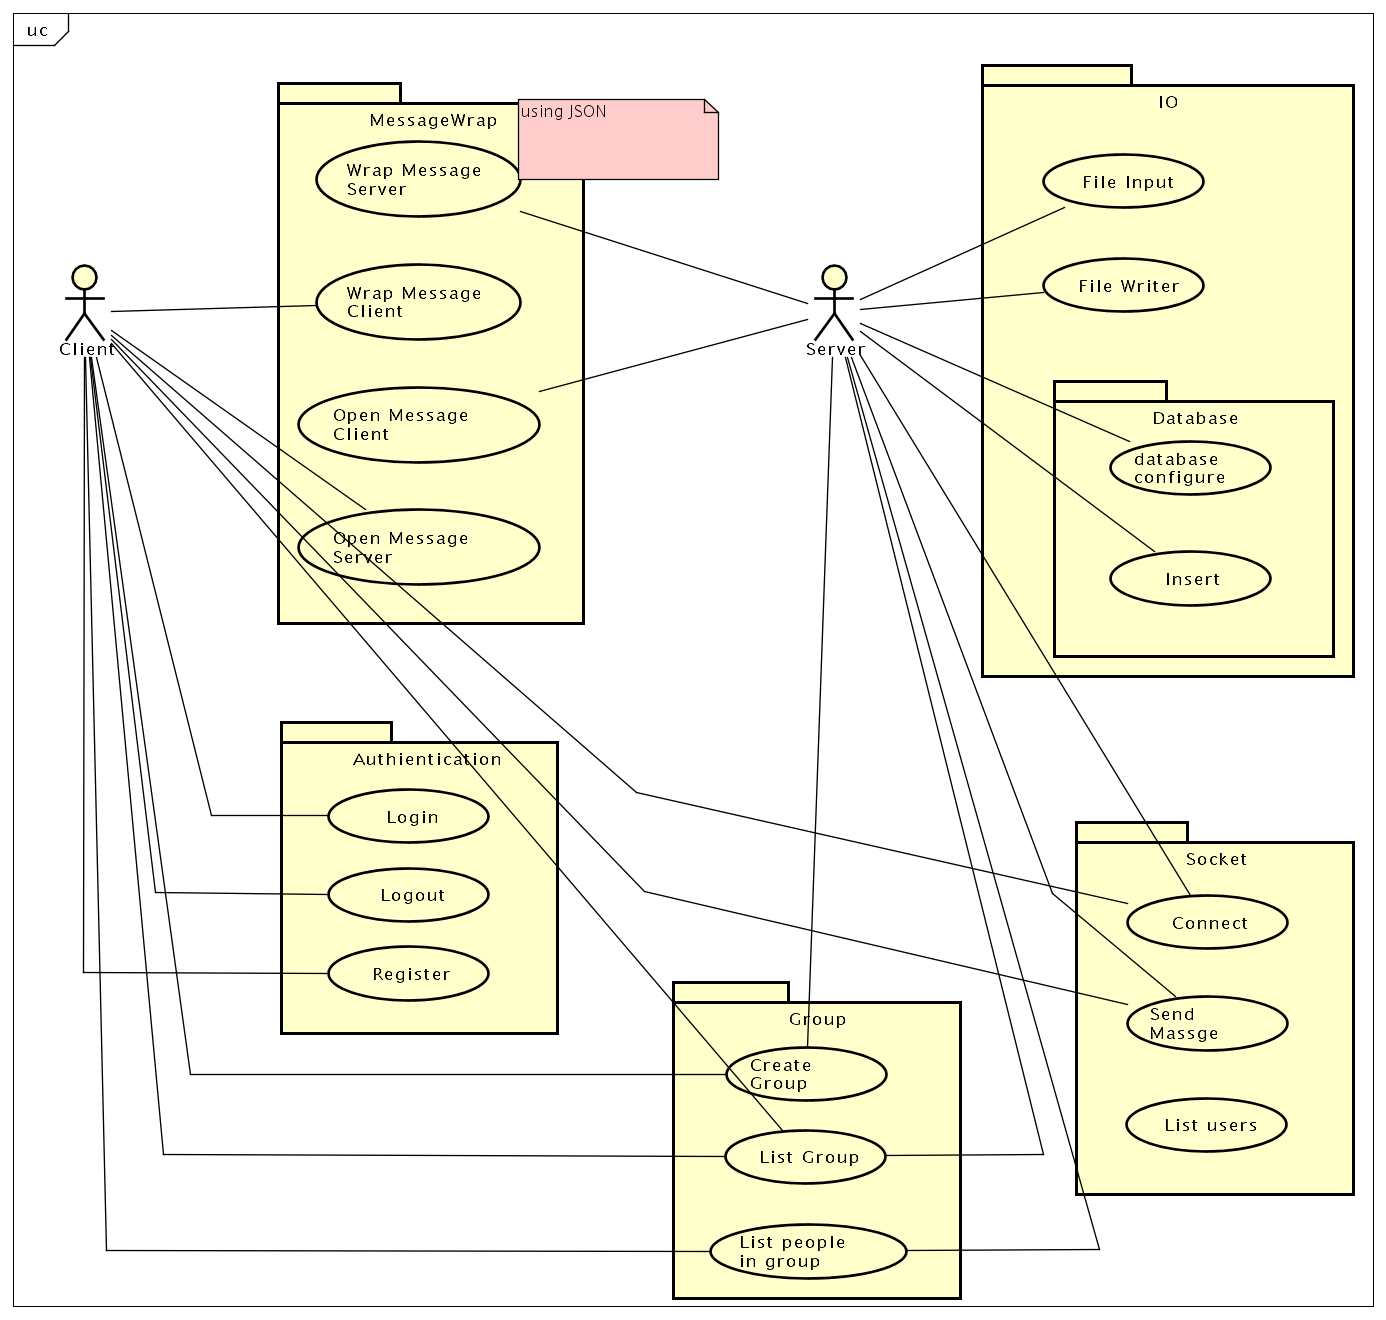
\includegraphics[scale=0.2]{usecase.png}
\caption{Module Design - Use Case diagram}
\end{figure}
\end{frame}

\begin{frame}{Log In}
\begin{figure}
	\begin{center}
		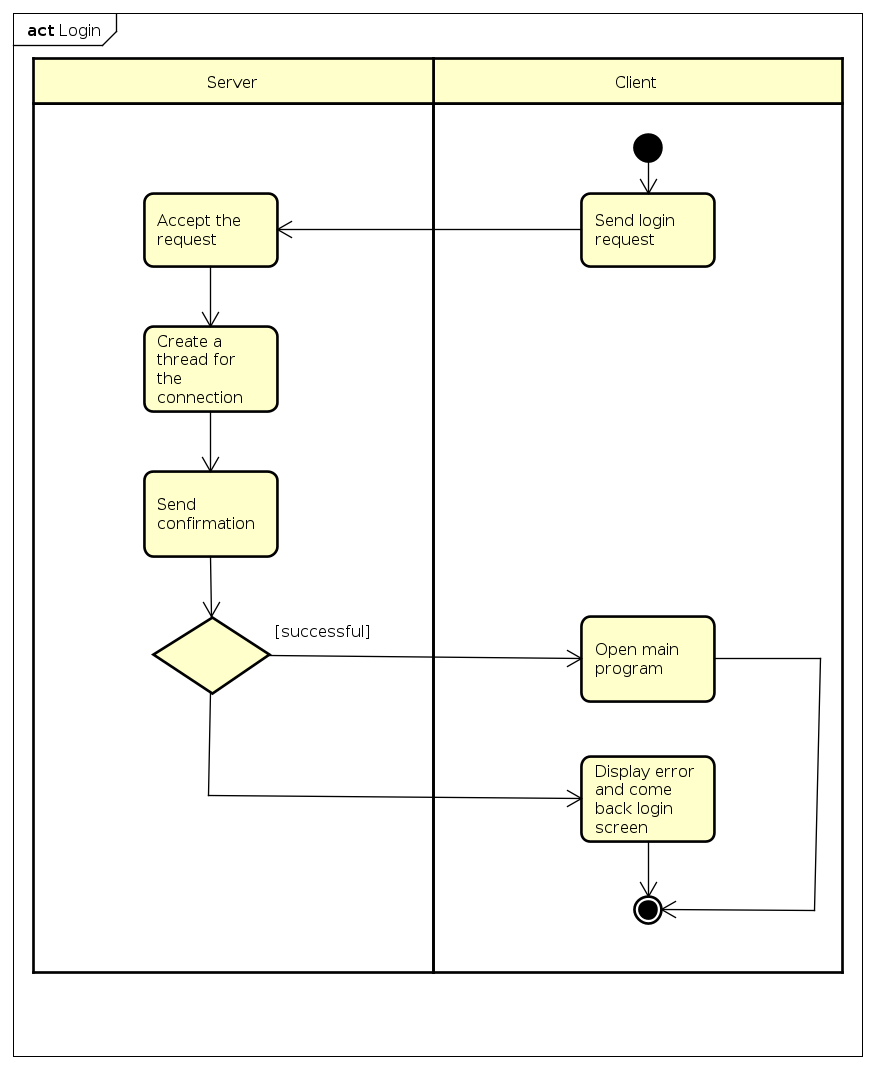
\includegraphics[scale=0.2]{Login.png}
		\caption{Log In - Activity diagram}
	\end{center}
\end{figure}
\end{frame}

\begin{frame}{Register}
\begin{figure}
	\begin{center}
		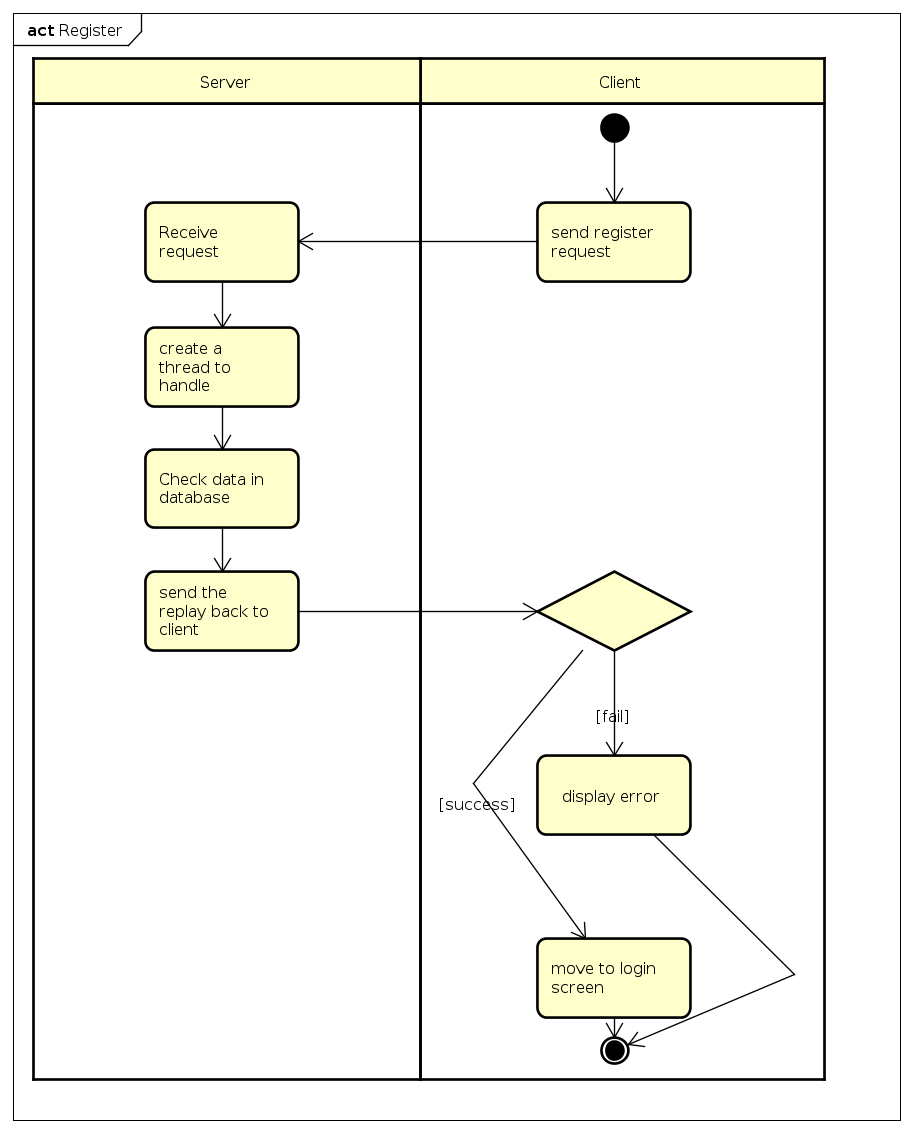
\includegraphics[scale=0.2]{Register.png}
		\caption{Register - Activity diagram}
	\end{center}
\end{figure}
\end{frame}

\begin{frame}{Send Messages To A Group}
\begin{figure}
	\begin{center}
		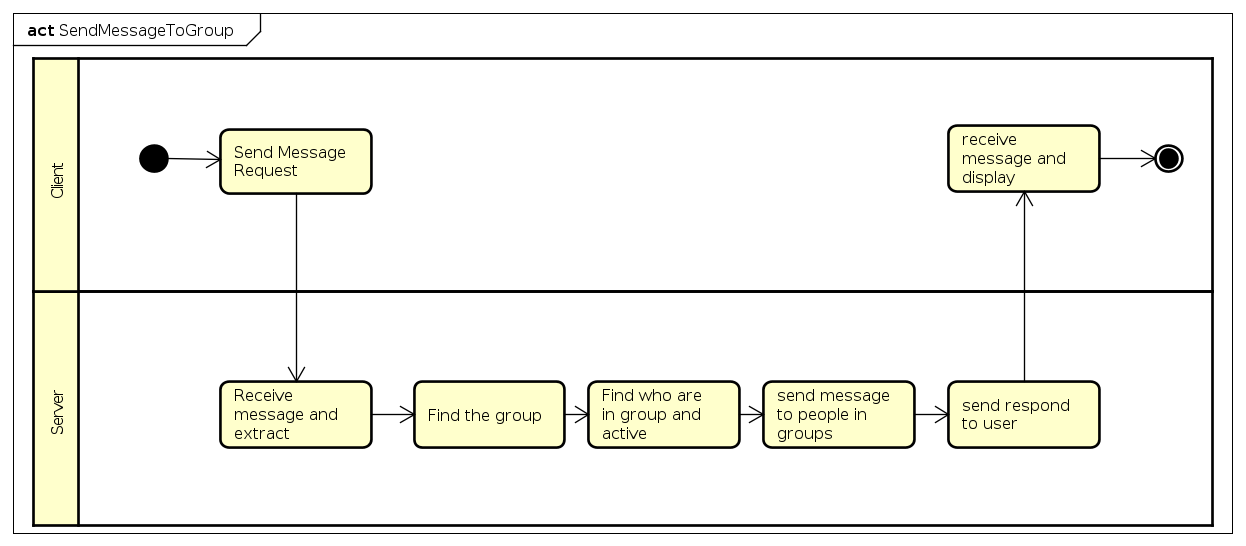
\includegraphics[scale=0.3]{SendMessageToGroup.png}
		\caption{Send message to group - Activity}
	\end{center}

\end{figure}
\end{frame}

\begin{frame}{Send Message To A Person}
\begin{center}
	\begin{figure}
		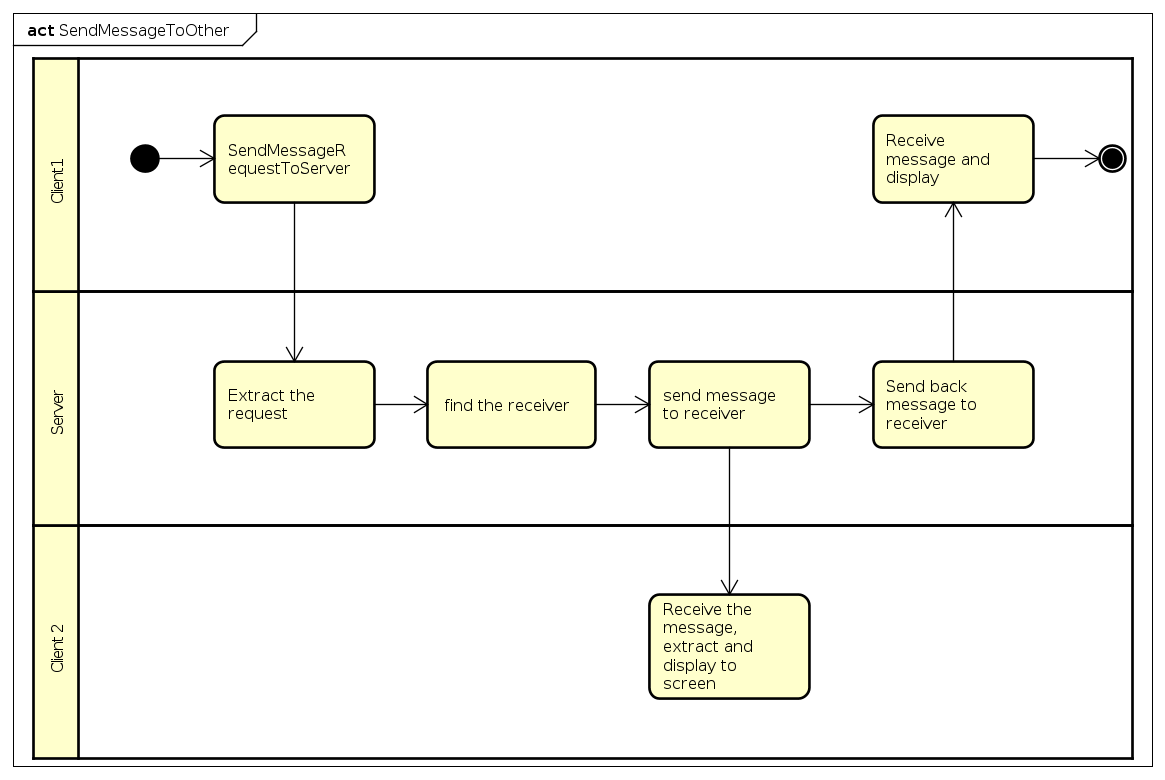
\includegraphics[scale=0.3]{SendMessageToOther.png}
		\caption{Send Message to an user}
	\end{figure}
\end{center}
\end{frame}
 
\section{Implementation Details}
\subsection{Data Structure}
\begin{frame}{Data Structure - Individual Chat}

\begin{itemize}
	\item Online Tree Represenation
	\begin{itemize}
		\item The online tree is a binary search tree
		\item Each online user will have a node on the tree
	\end{itemize}
\end{itemize}

\begin{center}
	\begin{figure}
		\includegraphics[scale=0.4]{OnlineTree.png}
		\caption{Online Tree Representation}
	\end{figure}
\end{center}
\end{frame}


\begin{frame}{Data Structure - Individual Chat}
	\begin{itemize}
		\item Online node representation
	\end{itemize}
	
	\begin{figure}
		\includegraphics[scale=0.4]{OnlineNode.png}
		\caption{Online Node representation}
	\end{figure}
\end{frame}

\begin{frame}{Data Structure - Individual Chat}
	\begin{itemize}
		\item Between 2 online nodes
		\begin{itemize}
			\item The message queue representative for the messages sending from node $1$ to node $2$.
		\end{itemize}
	\end{itemize}
	
	\begin{figure}
		\includegraphics[scale=0.4]{messageQueue.png}
		\caption{Message Queue between 2 online nodes}
	\end{figure}
\end{frame}

\begin{frame}{Data Structure - Group Chat}
\begin{itemize}
	\item Group Tree Representation
	\begin{itemize}
		\item Every group has 1 node on tree.
	\end{itemize}
\end{itemize}

\begin{figure}
	\includegraphics[scale=0.4]{OnlineTree.png}
	\caption{Group Representative Tree}
\end{figure}
\end{frame}

\begin{frame}{Data Structure - Group Chat}
\begin{itemize}
	\item Between 2 a group node and an user node
	\begin{itemize}
		\item The message queue representative for the messages sending from a person to a group
	\end{itemize}
\end{itemize}

\begin{figure}
	\includegraphics[scale=0.4]{GroupQueue.png}
	\caption{Message Queue for an user}
\end{figure}
\end{frame}


\subsection{Thread}
	\begin{frame}{Server}
		\begin{itemize}
			\item main thread for connection request
			\item 2 threads for each client
			\begin{itemize}
				\item 1 thread for listening message from client
				\item 1 thread for interacting with logic in server
			\end{itemize}
		\end{itemize}
	\end{frame}

\begin{frame}{Client}
\begin{itemize}
	\item Client will hold 2 threads
	\begin{itemize}
		\item 1 thread for receiving message from server
		\item 1 thread for taking order from client and sending message.
	\end{itemize}
\end{itemize}
\end{frame}






\end{document}
